%!TEX program = xelatex 
\documentclass{article} 
\usepackage{xunicode, xltxtra,xeCJK, ctex, graphicx} 
%简单来说,这个过程就像是Python里面的import和C语言里面的include。
% graphicx 图标包
% 语法:\includegraphics[options]{name}
\graphicspath{{figures/},{pics/}} % 图片放在当前目录下的figures和pics目录

\title{My First Document} 
\author{Wilson79} 
\date{\today}

\begin{document} 
	\tableofcontents % 产生文档目录,包括页码(非必需)
	\maketitle %制作封面

	% 可选参数[]可以不加,后缀也是可加可不加
	\includegraphics[scale=0.6]{mac1.png} 
	% scale整个图按比例缩放

	\includegraphics{mac2}
	
	\includegraphics[scale=0.7, height=8cm]{mac3}

	\includegraphics[scale=0.7, height=0.4\textheight, width=0.6\textwidth]{mac3} 
	% height=0.4\textheight 原图高度的0.4倍


	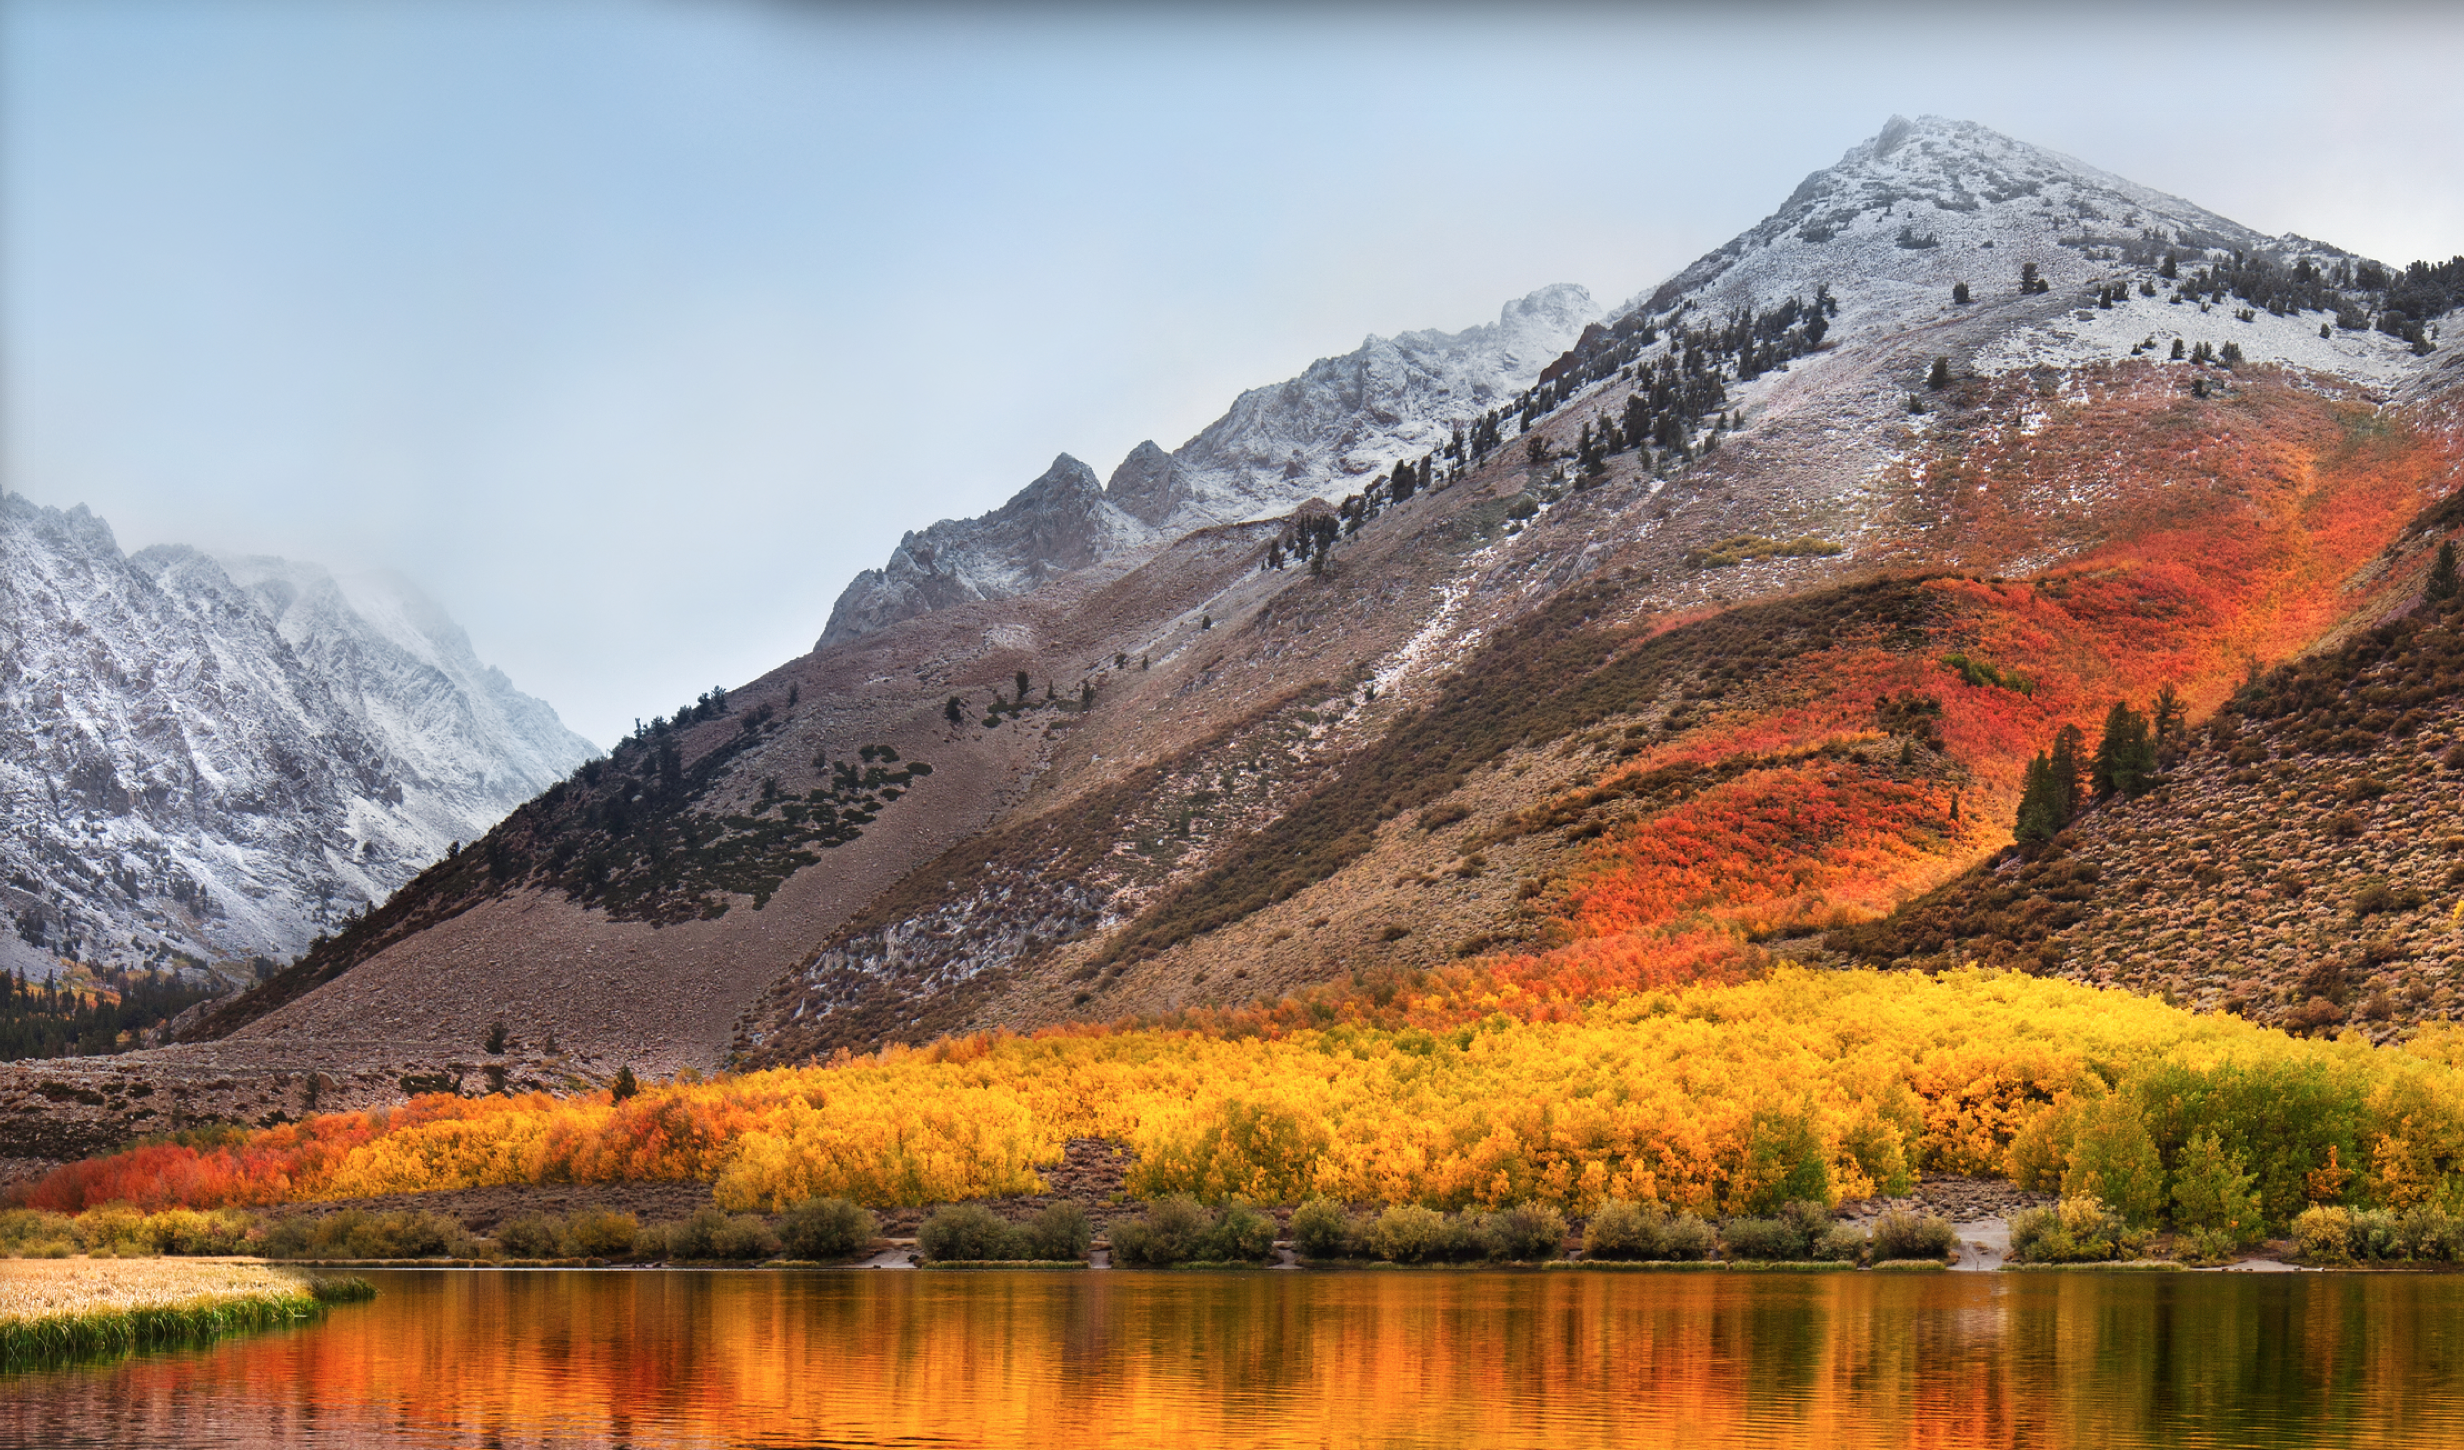
\includegraphics[angle=45, height=0.6\textheight, width=0.6\textwidth]{3232.png} 

	
	\section{LaTeX控制符} 
	\# \$ \% \} \^{}  \& \textbackslash %因为\\表示了换行不缩进,所以用\textbackslash来表示\

	\section{排版符号} 
	\S \P \dag \ddag \copyright \pounds

	%基本符号
	\TeX{} \LaTeX{} \LaTeXe{} % 暂时不明白后面为什么要加大括号

	\section{引号}
	` ' ``你好'' % 1左边的`, 加上enter左边的'
	\section{连字符} %子小节
	- -- ---
	\section{非英文字符} 
	\oe \OE \ae \AE \aa \o \O
	\section{重音符号} %子小节
	\`o \^0 \u{o} \r{o}


\end{document}

LaTeX图片
帮助文档  texdoc graphicx

LaTeX空白字符
1. 空格对中文不起作用,会被忽略,空格对英文起作用,多个空格等同于一个
同时英文夹在中文之间会自动在开头和结尾加上空格

可以用\ 来添加空格 到时候用的时候查手册就可以了,现在不需要特别记忆

2. 段落的首行缩进是自动产生的,绝对不能用空格替换
3. 空行分段,多个空行等同于一个